\section{Introduction}
Early, computer graphic got the ambition the produce photo realistic images.

Ray tracing is a way to produce visual images. The main advantage of this technique among others is the photorealism of produced image.

To produce an image, a ray tracing engine trace the reverse path of the light, from the virtual eye (camera) through a virtual screen (the image) and calculate the color of visible objects. You can see an example on the figure \ref{img_intro}.

\begin{figure}[ht]
  \centering
  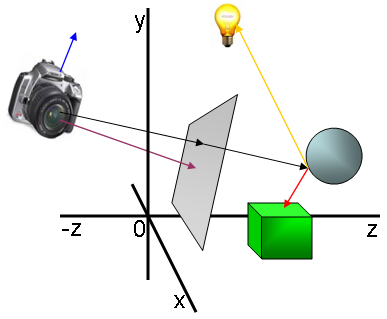
\includegraphics[height=7cm]{img/intro.png}
  \caption{Ray tracing}
  \label{img_intro}
\end{figure}

The eye (camera) look at a direction (purple arrow). A ray is traced through each pixel of the image (black arrow). The engine will try to find out where the ray intersect with an object (the sphere). The engine will find the color for this intersection by looking for the light and eventually reflexion of other objects (the cube).

